\section{Data and Model Specification}\label{sec:Data}
%quantities such as a monetary policy surprise measure , stock market returns, financial conditions and bilateral nominal exchange rates are stored in an $M\times 1$ vector $\bm y_t = (z_{EA, t}, \bm{f}_t, Stocks_t, CISS_t, FX_t)$ 
To examine high-frequency financial market reactions, we measure the impact of ECB monetary policy at a weekly frequency. This approach minimizes the noise typically present in daily time series, while still providing a sufficient number of observations for reliable inference beyond standard monthly frequencies. \rev{Our time series data span from $2005$:W$1$ to $2025$:W$52$, covering the pre-crisis boom, the global financial crisis, the euro area sovereign debt crisis, the long spell at the effective lower bound, the COVID-19 pandemic, and --- importantly for our question --- the post-pandemic global tightening cycle of 2022--2024, during which the Fed adopted a decisively restrictive stance outside a recessionary environment. Because the euro area inflation-linked swap panel now extends over the entire sample period, we estimate the full system---bond yields, inflation swaps, and the macro-financial block---jointly on this single sample, from which we obtain all headline yield, inflation-swap, and real-rate results.} Our ST-VAR model has a lag length of $p=4$, which captures dynamic dependencies up to one month in the past.  We start with the specific composition of the vector $\bm y_t$. For details on variable definitions, sources, and transformations, see \autoref{app:0}. We continue with an elaboration of the yield- and inflation-linked swap data and the respective estimated factors, and proceed with a description of the ECB's policy surprise measure and the Fed's policy stance.

\subsection{Estimation of the Yield and Inflation Swap Curve}

In our empirical work, we focus on macro-financial developments and monetary policy effects in the euro area, thus treating it as our home economy. Given the dominant role of US monetary policy in the global financial cycle, we condition \citep{miranda2020us, dees2021global} on the monetary policy stance of the Fed. Thus, the vector of observables $\bm y_t = (z_{EA, t}, \bm{f}_t, Stocks_t, CISS_t, FX_t)$ includes the monetary policy surprise instrument for EA ($z_{EA, t}$), the yield, indexed with $r$ and the inflation swap curve indexed with $\pi$ factors, $\bm f_t = (L_{rt}, S_{rt}, C_{rt}, L_{\pi t}, S_{\pi t}, C_{\pi t})$, and macro-financial time series for the EA. The latter consists of the EuroStoxx50 ($Stocks_t$), the Composite Indicator of Systemic Stress ($CISS_t$), and the USD-EUR exchange rate ($FX_t$). Our signal variable ($z^{\ast}_t$) is a measure of the US monetary policy stance. 

To construct the Nelson-Siegel factors of the yield curve, our weekly data set includes EA government bond yields (measured by yield curve instantaneous forward rates and labeled as \texttt{YLD}) for $15$ maturities, with $\tau \in \{1:10,12,15,20,25,30\}$.\footnote{In principle there are more maturities available within this continuum. However, to match the available maturities for the inflation swaps, we omit these. Including all accessible maturities for the government bond yields leaves the results virtually unchanged.} More specifically, we use only data compiled from AAA-rated bonds, as we want to avoid yield curve dynamics stemming from idiosyncratic country risks. During the euro area sovereign debt crisis, especially Greek, Italian, and Spanish government bond dynamics were subject to strong sovereign shocks. Hence,  an inclusion of all EA-bonds may impede the identification of monetary policy shocks as it becomes harder to distinguish policy from country-specific shocks. 

%To construct the Nelson-Siegel factors of the yield curve, our weekly dataset includes EA government bond yields (measured by the yield curve's instantaneous forward rates and labeled \texttt{YLD}) for $15$ maturities, with $\tau \in \{1:10,12,15,20,25,30\}$.\footnote{In principle, there are more maturities available along this continuum. However, in order to match the available maturities for the inflation swaps, we omit them. Including all available maturities for government bond yields leaves the results virtually unchanged.} More specifically, we use only data compiled from AAA-rated bonds, as we want to avoid yield curve dynamics driven by idiosyncratic country risks. During the euro area sovereign debt crisis, the dynamics of Greek, Italian, and Spanish government bonds in particular were subject to strong sovereign shocks. Therefore, including all EA bonds may complicate the dynamic analysis by making it more difficult to distinguish policy from country-specific shocks.

%Second, as mentioned in \cite{altavilla2019measuring}, the employed monetary policy surprise factors are constructed to only load on safe euro area assets. Therefore, the inclusion of individual country yields in our analysis would require a different set of monetary policy surprise instruments. \textbf{ich kapier das nicht wirklich.}

For obtaining the Nelson-Siegel factors of the inflation-linked swap curve, we consider EA inflation swaps (labeled as \texttt{INFSWP}) for 15 maturities matching those we used to construct the Nelson-Siegel factors above. More precisely, these are zero-coupon inflation swaps linked to the \rev{Harmonized Index of Consumer Prices (HICP)} excluding tobacco for the euro area. They depend on realized and expected inflation and can thus be employed as a hedging tool against future inflation. For our purposes they carry valuable information about \rev{market-based} expected future inflation, as reported in \cite{boraugan2020term} and discussed above.
It is important to note that inflation and inflation expectations have a significant impact on the real return that an investor can accumulate over time. In particular, future inflation represents a significant upside risk to real returns, against which investors can use ILS to protect against future inflation. Consequently, we use these swaps as a market-based proxy for otherwise latent inflation expectations. However, ILS also contain an \textit{inflation risk premium}, which investors invested in nominal assets demand for the arising inflation risks as well as a liquidity premium. In principle, to obtain the "pure" expectational component out of the swaps, one has to estimate a model and purge these swaps from other factors. However, for our application, we are interested in the composite, i.e., the inflation-linked swap per se, which includes a measure for uncertainty.  Moreover, ILS provide better information than other market-based measures (e.g., inflation-indexed Treasury yields), as shown by \citet{haubrich2012swaps}, and are similar to professional forecasters' expectations but less similar to households' inflation expectations. Since we are interested in high-frequency dynamics, survey-based expectations, typically at monthly or quarterly frequency, cannot be used. Therefore, we do not opt for an approach to disentangle "pure" expectations from the risk premium in market-based measures of inflation expectations. 


%%% REVISION: the near-verbatim repetition of the preceding ILS paragraph (flagged by both referees) has been deleted.

%Moreover, the swap price could also change due to increased inflation uncertainty and the need for higher uncertainty compensation, which is not necessarily linked to a change in the expectations. Nevertheless, ILS provide better information than other market-based measures (e.g., inflation-indexed treasury yields) as shown by \citet{haubrich2012swaps}. 

In addition to government bond yields and inflation swaps, we consider the nominal EUR-USD exchange rate (\texttt{FX}, in percentage changes) and the Euro Stoxx 50 index as a stock market indicator (\texttt{Stocks}, in percentage changes).  Thus, a depreciation of the exchange rate corresponds to an appreciation of the euro. We also include the EA composite indicator of systemic stress \citep[\texttt{CISS},][]{kremer2012CISS}. This index captures 15 indicators of stress in financial markets, and thus should be able to capture financial stability issues associated with monetary policy shocks. Finally, we differenced the data to ensure stationarity. %That is, the one Euro per US-dollar, such that a decrease denotes an appreciation of the Euro.

 

This dataset covers the financial side of the euro area economy in a high-frequency fashion. A key contribution of our analysis is thus the modeling of the full yield curve, which allows us to trace the effects of monetary policy on different (sub)segments of the EA yield curve. Moreover, since these quantities are nominal, the inclusion of the full inflation swap curve allows us to compute the corresponding real interest rate responses. This setup allows us to gain unique insights into how monetary policy affects not only nominal quantities, but also real quantities and inflation expectations. The inclusion of the CISS and the Eurostoxx index allows us to track movements in financial conditions. Finally, to capture the exchange rate-related channel of monetary policy, we also include the bilateral nominal exchange rate.

Next, we discuss the estimated yield curve and inflation swap curve factors.  Panels (a) and (b) in Figure \ref{fig:dataNS} show the respective Nelson-Siegel factors of the yields and inflation swaps in levels. As shown in panel (a), the variation in the curvature factor, $C_{rt}$, is considerably higher than that of the slope, $S_{rt}$, and level factors, $L_{rt}$, which is a common feature of yield curve factors. The negative slope factor throughout most of the sample reflects the typical upward pattern of the EA yield curve, except for short periods prior to the financial crisis, and surprisingly shows a negative correlation with the curvature factor. Towards the end of the sample, the increasing (but still negative) slope factor indicates a flatter curve.
In addition, we observe that the level factor fluctuates around a long-run level of about $5\%$ before the financial crisis, but falls sharply in the middle of the crisis, with a steady decrease in the trend of long-term nominal interest rates in subsequent periods and in the aftermath of the Great Recession. This reflects a secular decline in long-term yields, driven in part by unconventional monetary policy in the EA and lower levels of trend inflation. \rev{This decline reverses at the end of the extended sample: the level factor bottoms out around 2020 and then rises markedly during the 2022--2024 tightening cycle, recovering to roughly $3$--$4\%$ as policy rates and long-term yields normalized in the wake of the post-pandemic inflation surge.} The slope and curvature factors tell a similar story, and the movements can again be linked to monetary policy.

\begin{figure}[!htpb]
\centering
\caption{Yield curve and inflation swap factors for the EA. \label{fig:dataNS}}
\begin{minipage}{\textwidth}
\centering
a) Yield curve factors
\end{minipage}
\begin{minipage}{\textwidth}
\centering
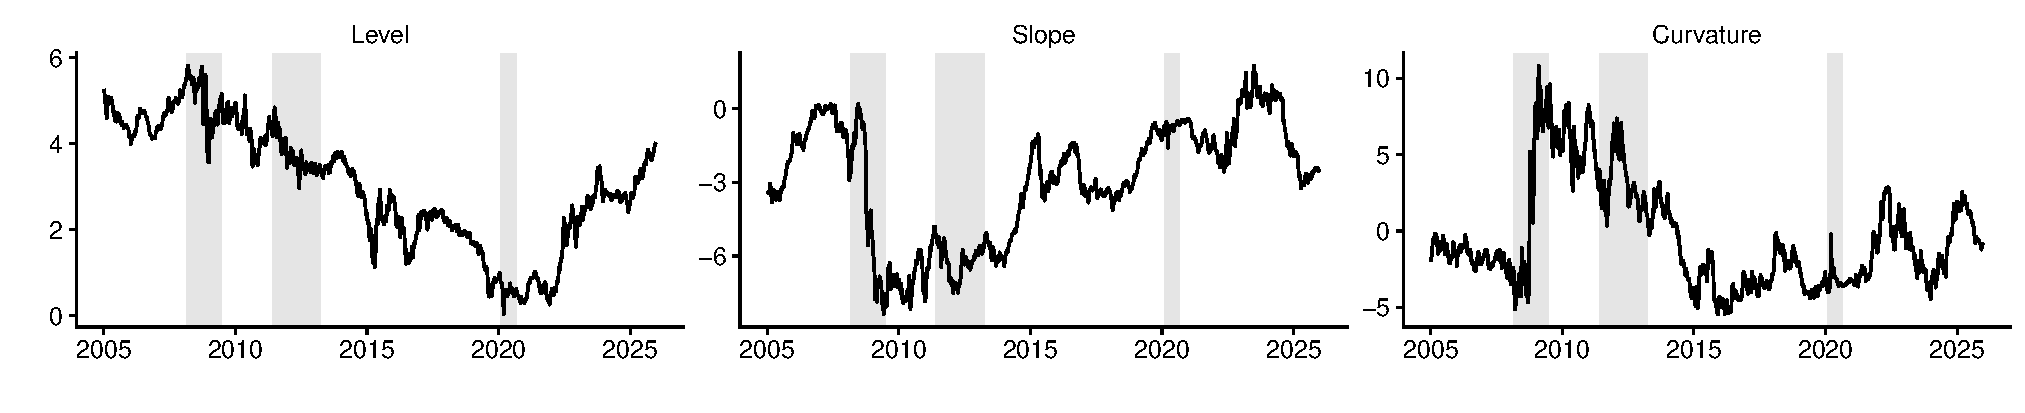
\includegraphics[width=1\textwidth]{images_updated/descript/YLD_NSfacs.pdf}
\end{minipage}
\begin{minipage}{\textwidth}
\centering
\vspace{5pt}
b) Inflation swap curve factors
\end{minipage}
\begin{minipage}{\textwidth}
\centering
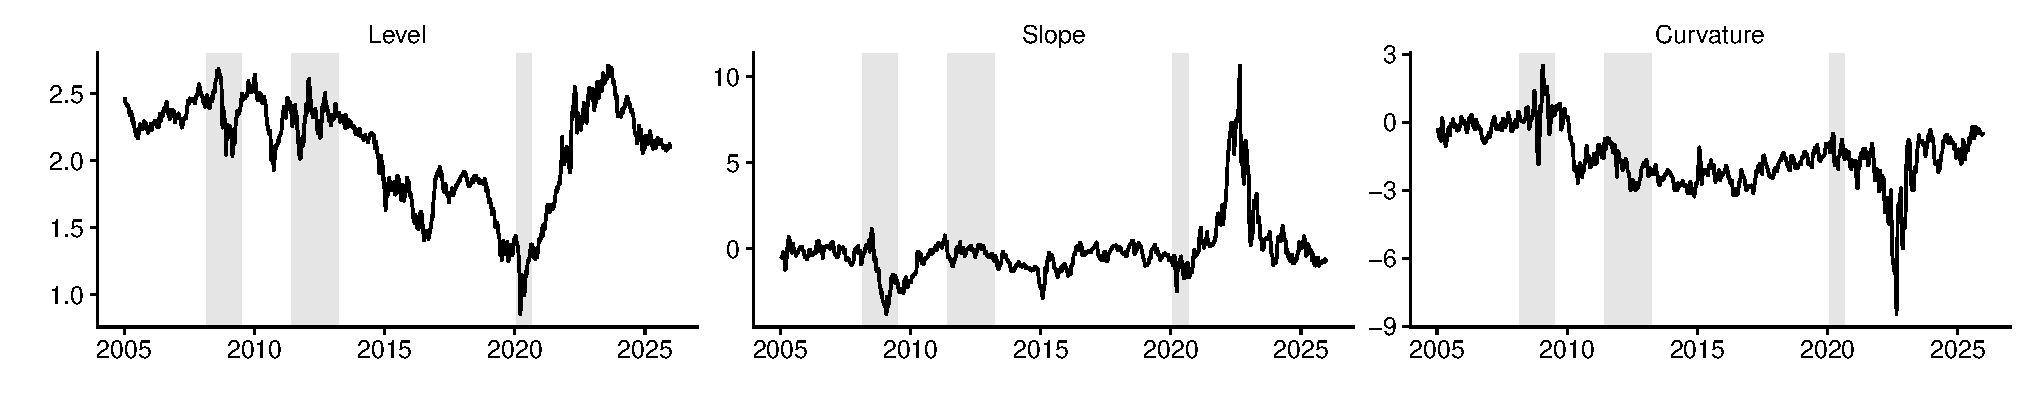
\includegraphics[width=1\textwidth]{images_updated/descript/INFSWP_NSfacs.pdf}
\end{minipage}
\caption*{\textit{Notes:} The factors (shown in levels) are obtained with a three-factor Nelson Siegel model, where $L_{jt}$ can be interpreted as the level, $S_{jt}$ as the slope, and $C_{jt}$ the curvature factor for $j$ being either the associated yield curve ($r$) or the inflation swap curve ($\pi$) factors. Gray shaded areas indicate EA recessions based on the Euro Area Business Cycle Dating Committee. \rev{Factors are shown for the full $2005$--$2025$ sample.}}
\end{figure}

Turning to the estimated factors associated with the inflation swap curve, other interesting findings emerge. First, we find a substantial and persistent decline in the level of inflation expectations \rev{over the first two-thirds of the sample, which subsequently reverses}. Given the level of the yield curve in panel (a) of Fig. \ref{fig:dataNS}, this suggests that real interest rates were positive and then approached negative territory \rev{around 2020. With the post-pandemic inflation surge, however, both nominal yields and inflation swaps rebounded sharply, so that by the end of the sample real interest rates had returned to clearly positive territory}. Both the slope and the curvature of the swap curve show a sharp decline during the global financial crisis. This implies that short-run inflation expectations declined, while long-run inflation expectations either remained constant or increased. Interestingly, a second sharp decline in the slope of the swap curve is observed during the introduction of the Asset Purchase Program (APP) in mid-2014. This and subsequent purchase programs were designed to support the ECB's policy in the face of the effective lower bound. However, \cite{burban2021ILSrisk} provide a decomposition of the ILS into its expectation and risk premium components. Their estimates suggest a change in the sign of the risk premium around 2013/2014. Therefore, this dynamic could also be reflected in our results. After another significant decline in early 2015 to 2016, possibly caused by another round of asset purchases, the slope fluctuates around zero, implying rather stable inflation expectations over different horizons. \rev{This stability breaks down at the end of the extended sample: during 2021--2022 the slope factor of the swap curve spikes sharply, reflecting a pronounced rise in short-horizon relative to long-horizon inflation expectations as headline inflation surged, before receding as the surge faded and expectations re-anchored.} To ensure stationarity, the respective factors are differenced in the estimation.

\subsection{Measuring Monetary Policy}\label{sec:measuring}
In order to detect monetary policy interactions between the US and the euro area, we rely on a unique measure of ECB monetary policy shocks, which renders a separate identification obsolete. Moreover, we use an instrument that is purged of various types of shocks and thus carries only information about monetary policy itself. As shown in \cite{jarocinski2020deconstructing}, central bank communication conveys information not only about monetary policy but also about the state of the economy. This so-called information effect can cause adverse reactions on financial market variables. Therefore, for our purpose of analyzing the effects of monetary policy, we need to make sure that the instruments used are clearly related to monetary policy surprises.
%It is worth mentioning that our  sample covers the zero lower bound episode and thus the implementation of unconventional monetary policy measures. Hence, our surprise series needs to incorporate sufficient information about surprises not stemming from conventional policy actions. Indeed, the choice of the respective monetary policy surprise series may be crucial for the consecutive analysis, such that we provide several robustness checks in \autoref{sec:results_rob}.

A convenient measure of EA monetary policy shocks (i.e., our domestic shocks, $z_{EA,t}$) that satisfies the above requirements has been proposed in \cite{altavilla2019measuring}. This measure is based on the Euro Area Monetary Policy Event-Study Database and exploits the high-frequency reactions of financial markets in a narrow window (ten minutes before and after the event) around identified events associated with monetary policy announcements.\footnote{The full Event-Study Database can be found via \href{https://www.ecb.europa.eu/pub/pdf/annex/Dataset_EA-MPD.xlsx}{https://www.ecb.europa.eu/pub/pdf/annex/Dataset\_EA-MPD.xlsx} and a detailed description of the methodology and data  in \cite{altavilla2019measuring}.} 
The extracted factors consist of the target, the timing, the forward guidance, and the quantitative easing factor, respectively. Each of these factors has an impact on different segments of the yield curve. %Since we are interested in a comprehensive identified measure of monetary policy surprises, we consider a linear combination of these factors.
By taking the sum of these factors, we obtain a broad summary measure of monetary policy surprises.\rev{\footnote{We use the regularly updated factor estimates maintained by Giuseppe Ragusa (\href{https://gragusa.org/factors/}{https://gragusa.org/factors/}, vintage October 2025), which apply the methodology of \cite{altavilla2019measuring} to the current Euro Area Monetary Policy Event-Study Database. Since the factors are re-estimated on the full sample in each vintage, point estimates differ marginally across vintages, with correlations above $0.98$.}} To avoid a contamination of this unified measure with information effects, we use the approach introduced in \cite{jarocinski2020deconstructing}, called "poor-man's sign restrictions". This is achieved by restricting the stock market reaction to policy shocks to be negative in sign. This restriction ensures that we have a measure that only captures monetary policy surprises. \rev{Moreover, \cite{altavilla2019measuring}, Appendix A, flag three announcements (August 31, 2006, October 8, and November 6, 2008) at which no press conference followed the Governing Council meeting, so that the second event window used to identify the timing, forward guidance and quantitative easing factors does not exist. In the vintage we use, two of these dates (October 8 and November 6, 2008) carry no factor values and therefore enter our weekly measure as zeros; the third (August 31, 2006) enters with a surprise of $+2.0$ basis points, negligible against the $5.7$ basis point standard deviation of the series, and we retain it.}

To measure the corresponding US monetary policy stance, denoted $z_t^\ast$, we use the effective federal funds rate, $DFF_t$, and subtract the (one-sided) natural rate estimate, $r^{\ast}$, obtained using the model proposed in \cite{laubach2003measuring}. Since the latter estimate is only available at the quarterly frequency, we use a linear interpolation to adjust it to the weekly frequency. The effective rate thus serves as a fast-moving component of the stance, while the natural rate captures slower trends. This measure allows us to interpret values above (below) zero as a tight (loose) US monetary policy stance. \rev{This constitutes our baseline stance measure. To ensure that our findings do not hinge on how the stance is measured---in particular on the treatment of the effective-lower-bound period, during which the federal funds rate is pinned near zero---we consider two model-based alternatives as robustness checks: the shadow short rate and the effective monetary stimulus of \cite{krippner2016ems}, each taken relative to $r^{\ast}$.}


%For the US monetary policy shocks $z_t^\ast$,  we use the instrument stipulated in \cite{bu2021unified}.We measure the US monetary policy stance through the  unified measure constructed by \cite{bu2021unified}.\footnote{The series can be downloaded via \href{https://www.federalreserve.gov/econres/feds/a-unified-measure-of-fed-monetary-policy-shocks.htm}{https://www.federalreserve.gov/econres/feds/a-unified-measure-of-fed-monetary-policy-shocks.html}.} This constructed shock series conveniently summarizes and quantifies conventional and unconventional monetary policy in the US. While also exploiting variations in a specific time window around FOMC meeting days, the extraction of surprises follows a \cite{famamacbeth1973FedMP} approach and takes periods of conventional and unconventional monetary policy equally into account. The advantages of this measure are twofold. First, the absence of a central bank information effect allows us capturing only the pure monetary policy shocks.  Second, it conveniently pictures US surprises during the zero lower bound episode. 

%For our consecutive analysis, we introduce some persistence to this measure by computing one-quarter ($13$ weeks) moving averages of the instrument. This facilitates interpretation as the Fed's monetary policy stance, since it summarizes unexpected shifts in monetary policy over a longer period of time. This transformed variable then serves as our threshold variable  $z_t^\ast$.  Hence, our measure of the US monetary policy stance is backward looking by about $13$ weeks, implying that shocks occurring in time $t$ impact  the regime allocation for the next $t+13$ periods. %This reflects the notion that monetary policy works with some lags. 

In \autoref{fig:dataMPshk} the monetary policy surprise instruments, $z_{EA,t}$, and the US monetary policy stance, $z_t^\ast$, are shown.\footnote{\rev{Two euro area surprises are exceptional in magnitude and are highlighted with red dots in \autoref{fig:dataMPshk}. We flag them here because both are contaminated by non-monetary-policy events and are therefore excluded, on economic grounds, from all of our estimates --- both the reduced-form pass-through regressions in \autoref{sec:passthrough} and the structural model of \autoref{sec:results}. This exclusion rests on our own judgement about the validity of the surprise and is distinct from the three no-press-conference announcements discussed above, which concern how the factors are constructed rather than how the surprise is interpreted. The first, on 17 March 2023 ($+30.7$ bps), coincides with the collapse of Silicon Valley Bank and the distress at Credit Suisse: the ECB raised rates by 50 basis points into an acute banking-stress episode, yet euro area yields \textit{fell} on a flight to safety, so the co-movement reflects financial-stress dynamics rather than the transmission of the policy surprise itself. The second, on 4 July 2008 ($-23.8$ bps), falls in the week of the ECB's final pre-crisis rate hike at the onset of the global financial turmoil, a period of severe money-market dislocation in which the high-frequency surprise is unusually large and hard to interpret as a clean policy shock. Exclusion is implemented differently in the two settings, for mechanical reasons: the event-week regressions of \autoref{sec:passthrough} drop the two observations from the estimation sample, whereas in the VAR of \autoref{sec:results} the weeks remain in the system and only the surprise itself is set to zero, so that they are treated as weeks without an ECB announcement. Deleting an observation outright is not available in a VAR, where the missing value would propagate through the lag structure and remove several consecutive weeks from every equation. The distinction is immaterial here. With the surprise set to zero, these weeks contribute exactly nothing to the first row and column of the residual covariance matrix, which is what determines the impact responses under our recursive identification; and they are not themselves outliers in the endogenous variables (17 March 2023 moved the ten-year yield by $0.8$ and the two-year yield by $0.1$ standard deviations), together accounting for less than $3\%$ of the residual variation.}} Several features stand out. From the beginning of our sample until the onset of the financial crisis, the Fed pursued a restrictive policy, reflected in a tight stance. To cope with the effects of the crisis, it cut policy rates sharply and introduced additional unconventional measures to counteract the downturn. Most importantly, these measures were designed to support the severely impaired interbank market to maintain liquidity in times of severe financial turmoil and to overcome the constraints imposed by the zero lower bound. The Fed continued its unconventional measures in the form of large-scale bond purchases. As a result, the stance remained rather accommodative until the first quarter of 2017, after which it shifted to a tighter stance given the intention to normalize the balance sheet. \rev{After a renewed easing around the COVID-19 shock, the stance rose sharply during the 2022--2024 tightening cycle, reaching its most restrictive readings of the entire sample.}
The ECB's policy surprises, on the other hand, reveal different information. While the period of the financial crisis was characterized by high upside and downside surprises, in early 2011 the ECB tightened its stance in two consecutive quarters. The benchmark interest rate (on the main refinancing operations) was set at 1.5\% in July, leading to large tightening surprises. Shortly thereafter, the euro area entered a recession, prompting the ECB to adopt a more expansionary policy, with expansionary surprises. In subsequent periods, the surprises have been mixed. \rev{Toward the end of the sample the transatlantic divergence becomes particularly pronounced: the Fed moved to the most restrictive stance of the entire sample during the 2022--2024 tightening cycle, while the euro area monetary policy surprises remained comparatively contained. It is precisely this configuration---a decisively tight Fed outside a euro area recession and away from the effective lower bound---that supplies much of the identifying variation exploited in the state-dependent analysis below.}


%After the financial crisis, in 2010, the euro area headed into a substantial sovereign debt crisis such that  the ECB's policy stance remains quite loose, however with a decreasing pace. In contrast, the Fed continued their bond buying programs at a large scale, represented by a much more pronounced decrease of the surprises. 

%The correlation between the euro area surprises and the Fed policy stance is -0.018 (p-value = 0.61) for the whole sample. 
%However, it might be the case that the correlation is increasing over time, which we check in panel (b) of \autoref{fig:dataMPshk}. Here we plot the rolling correlation between ECB and Fed monetary policy surprises with a one quarter (i.e., 13 weeks) window. The general picture supports the notion of not much coordination between the Atlantic in terms of policy surprises, as only four brief episodes reveal a bit stronger positive correlations, either within recessionary episodes or shortly before/after. This may be explained by the similar required central bank reaction to common shocks hitting both, the euro area and the United States simultaneously.


% \begin{figure}[!htpb]
% \centering
% \caption{Cumulative monetary policy surprises for both EA and US.\label{fig:dataMPshk}}
% 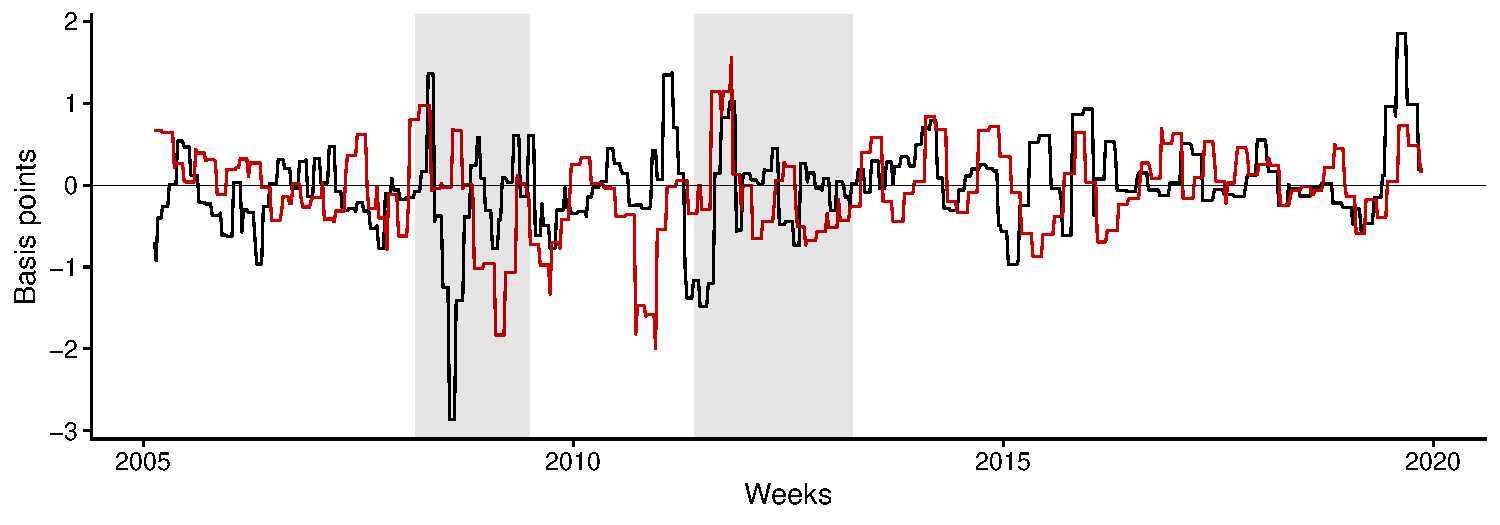
\includegraphics[width=1\textwidth]{images/descript/MPshks_surpr_MA13Motto-Bu.pdf}
% \caption*{\footnotesize \textit{Notes:} The black line denotes cumulative EA monetary policy surprises of \cite{altavilla2019measuring}, while the red line refers to cumulative US monetary policy surprises of \cite{bu2021unified} in basis points. Gray shaded areas indicate EA recessions based on the the Euro Area Business Cycle Dating Committee.}
% \end{figure}

\begin{figure}[htpb!]
\centering
\caption{EA Monetary policy surprises (black) and US monetary policy stance (\rev{blue}). \label{fig:dataMPshk}}
%\begin{minipage}{\textwidth}
%\centering
%a) Surprises smoothed with MA(13)
%\end{minipage}
%\begin{minipage}{\textwidth}
\centering
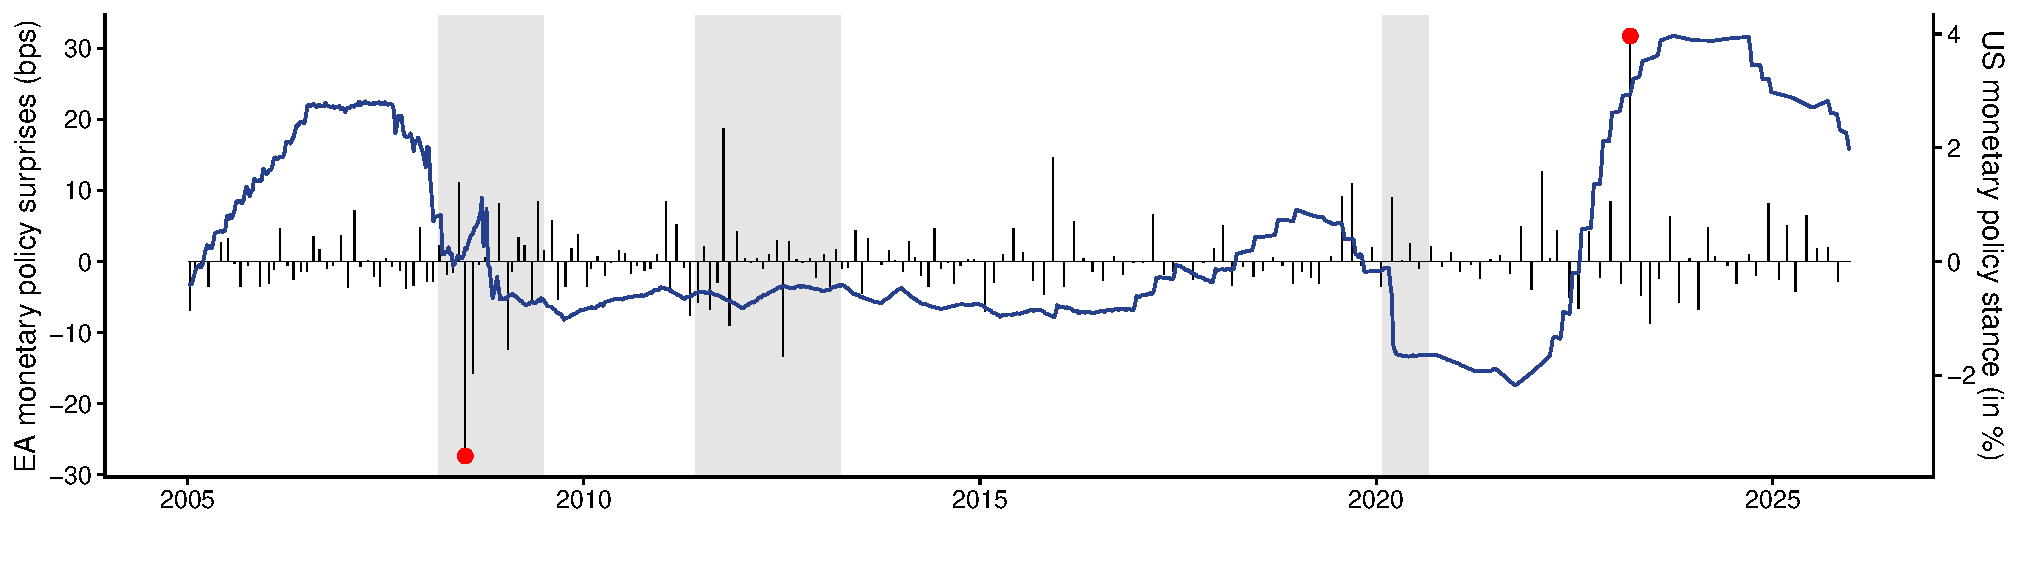
\includegraphics[width=1\textwidth]{images_updated/descript/MPshks_surpr_US_stance.pdf}
% \end{minipage}
% \begin{minipage}{\textwidth}
% \centering
% \vspace{5pt}
% b) Rolling correlation with one quarter (13 weeks) window between EA and US surprises
% \end{minipage}
% \begin{minipage}{\textwidth}
% \centering
% 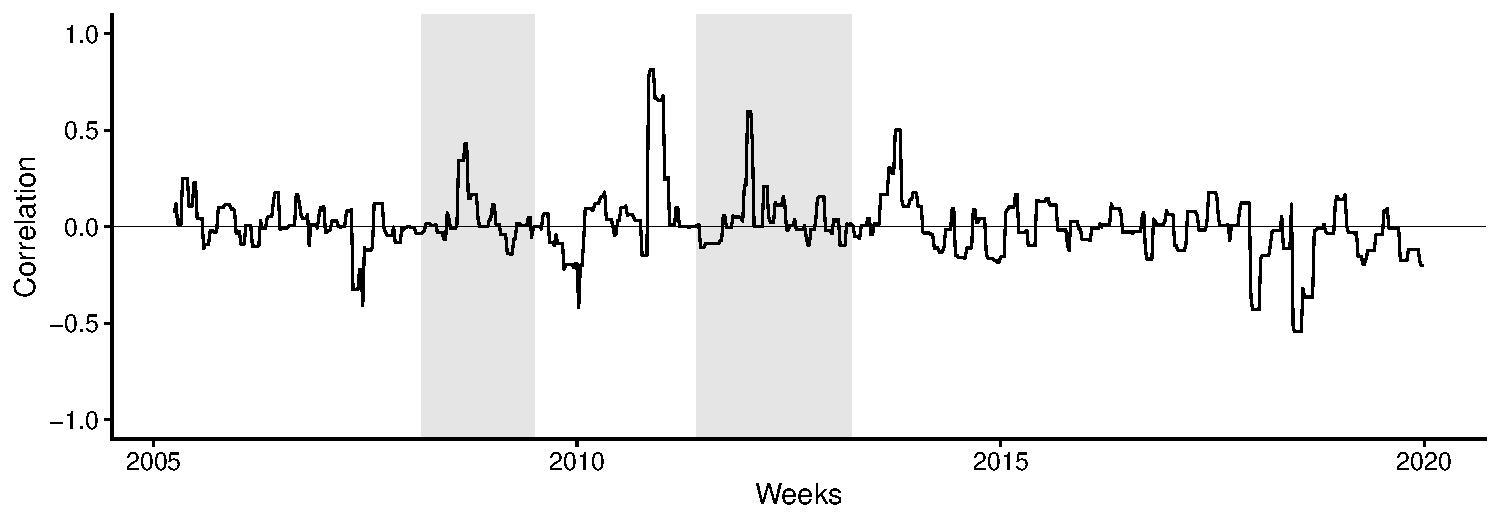
\includegraphics[width=1\textwidth]{images/descript/MPshks_surpr_MA13_rollcorrMotto-Bu.pdf}
% \end{minipage}
\caption*{\textit{Notes:} The black bars denote the EA monetary policy surprises of \cite{altavilla2019measuring}, while the \rev{blue} line refers to the US monetary policy stance ($DFF_t-r^{\ast}$). Gray shaded areas indicate EA recessions based on the Euro Area Business Cycle Dating Committee. \rev{The two red dots mark the two outlier surprises discussed in the text (17 March 2023 and 4 July 2008). Shown for the full $2005$--$2025$ sample.}}
\end{figure}




\subsection{\rev{Transmission of ECB surprises across the term structure}}\label{sec:passthrough}

\rev{Before turning to the dynamic model, we establish how euro area financial markets respond to an ECB monetary policy surprise, and we use the exercise to frame the central question of the paper. For each maturity $\tau$ we regress the weekly change in the nominal yield, and separately in the inflation-linked swap rate, on the euro area surprise,}
\begin{equation}\label{eq:passthrough}
    {\color{red} \Delta y^{\tau}_{t} = a_{\tau} + b_{\tau}\,\mathrm{MP.EA}_t + \varepsilon^{\tau}_{t},}
\end{equation}
\rev{and trace the estimated pass-through coefficient $b_{\tau}$ along the whole term structure. \autoref{fig:passthrough} plots $b_{\tau}$ (in basis points of yield per basis point of surprise) for all $15$ maturities, with $90\%$ confidence bands. Two ECB surprises are extreme outliers contaminated by contemporaneous financial-stress events; they are excluded from the baseline on economic grounds (see the discussion around \autoref{fig:dataMPshk}), and the dashed line shows that including them attenuates the estimates but leaves the maturity profile unchanged.}
\begin{figure}[ht!]
\centering
\caption{\rev{Pass-through of ECB monetary policy surprises along the term structure.}}\label{fig:passthrough}
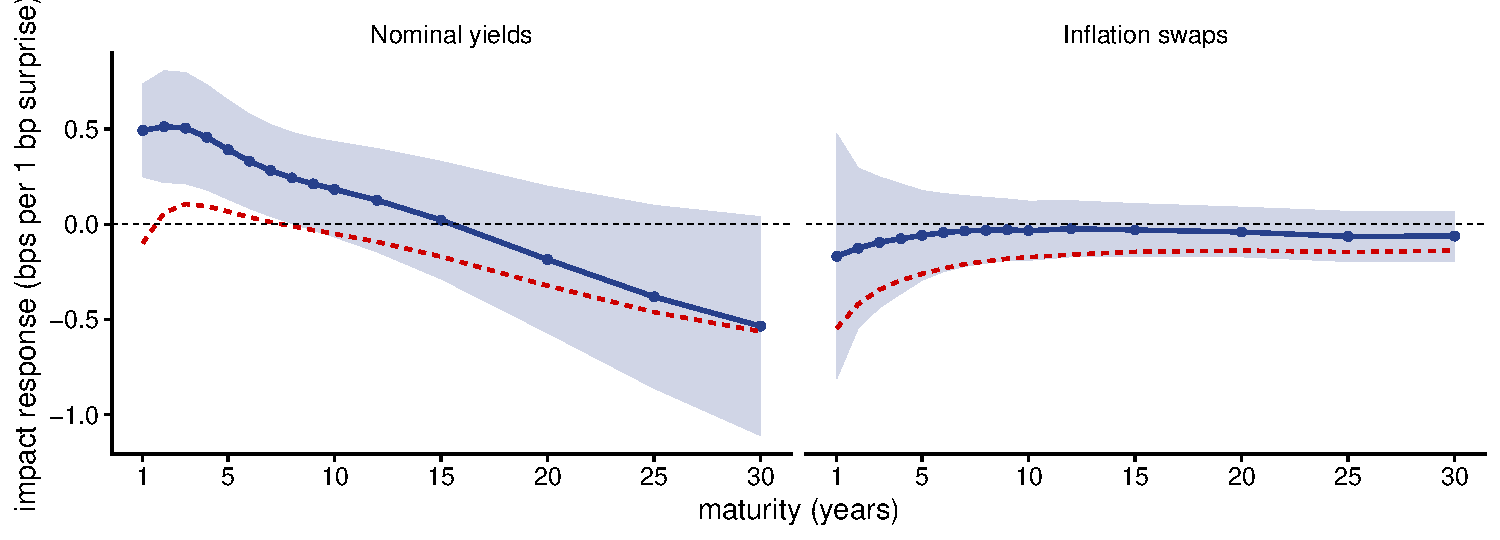
\includegraphics[width=\textwidth]{images_updated/passthrough_curve.pdf}
\caption*{\rev{\footnotesize \textit{Notes:} Each point is the slope coefficient $b_\tau$ from an event-week regression \eqref{eq:passthrough} of the weekly change in the nominal yield (left) or inflation-linked swap (right) of maturity $\tau$ on the euro area monetary policy surprise \citep{altavilla2019measuring}, expressed in basis points of yield per basis point of surprise. The solid line and shaded $90\%$ band exclude the two outlier surprises discussed in \autoref{sec:measuring} (17 March 2023 and 4 July 2008); the red dashed line includes all events. Heteroskedasticity-consistent standard errors; weekly data, 2005--2025.}}
\vspace{-3mm}
\end{figure}
\rev{Three features stand out. First, the surprise transmits strongly to \textit{nominal} yields at the short end: a one-basis-point tightening surprise raises the one- to three-year yield by about half a basis point ($t\approx 3$), an effect that declines monotonically with maturity and is indistinguishable from zero beyond ten years. Second, the response of inflation-linked swaps is negative but small and imprecisely estimated at all maturities, so the tightening is transmitted primarily to \textit{real} rates: the implied short-maturity real yield rises by roughly one-half to two-thirds of a basis point per basis point of surprise ($t\approx 2$). Third, the pattern is a genuine term-structure phenomenon --- transmission is concentrated at the maturities where conventional and forward-guidance policy operate and dissipates at longer horizons. Taken together, these facts confirm that our instrument captures economically meaningful, correctly signed monetary policy surprises, and they put to work the full yield and inflation-swap curves that are the empirical contribution of this paper.}

\rev{The question this paper is concerned with is whether this transmission depends on the stance of US monetary policy. Simple, model-free tools cannot answer it. Splitting the sample into loose- and tight-Fed weeks and running \eqref{eq:passthrough} separately, or estimating state-dependent local projections out to a quarter, yields loose- and tight-regime responses that are statistically indistinguishable at weekly frequency, and the little contrast that does appear is sensitive to individual high-leverage observations.\footnote{\rev{Across maturities and horizons the loose-versus-tight difference in the impact response is statistically insignificant, with $p$-values above $0.5$ once the two outlier surprises discussed in \autoref{sec:measuring} are excluded. These checks are available upon request.}} This is unsurprising: weekly financial data have a low signal-to-noise ratio, the exercise ignores dynamics, and a binary split coarsely discretizes a continuous stance. Answering the question convincingly requires a framework that pools information across the whole system, replaces the binary split with a smooth transition in the Fed's stance, allows for dynamics beyond the impact week, and disciplines the resulting parameter proliferation through shrinkage. This is precisely the smooth-transition VAR to which we now turn.}

%%% [REVISION 2026-07] The previous motivating exercise --- a scatter of first-differenced real 10-year
%%% yields split by the Fed stance (former Figure "fig:interaction", images/new_Regression_plot.pdf) and
%%% the accompanying Nelson-Siegel interaction regression (former Table "tab:regression") --- has been
%%% REPLACED by the term-structure pass-through analysis above. On the 2005-2025 sample the earlier
%%% sign-switch was not robust: it was driven by two outlier surprises (above all the SVB / Credit Suisse
%%% week of 17 March 2023). The retired equation, table and discussion are preserved but not typeset,
%%% inside the \iffalse ... \fi block below.
\iffalse

%As we showed in \autoref{fig:interaction} in the introductory section, there exists a considerably different effect of monetary policy shocks on the euro area 10-year real bond yields if we account for the respective Fed's policy stance. 

%After obtaining the \textit{full} yield and inflation expectation term structure by employing the constructed Nelson-Siegel factors of the respective curve (see \autoref{fig:dataNS}), we are able to take a closer look at which factors are affected most by interaction effects. In \autoref{tab:regression} we report the results of regressing the obtained yield and swap curve factors on the ECB's policy surprises  and the changes in the Fed's stance, as well as on the interaction between those instruments.

Specifically, we use our  constructed Nelson-Siegel factors of the nominal yield and inflation swap curve (see \autoref{fig:dataNS}) and estimate 
\begin{equation}\label{eq:univRegr}
    y_{it} = \beta_{i0} + \beta_{i1}\text{MP.EA}_t + \beta_{i2}\Delta\text{MP.US}_t + \gamma_{i} (\text{MP.EA}_t \times \Delta\text{MP.US}_t) + \epsilon_{it}
\end{equation}
where $i\in\{L, S, C\}$ denotes the level, slope, and curvature factor of the yields and swaps in their level values, MP.EA is the EA monetary instruments used, $\Delta$MP.US is the change in the Fed's policy stance, and $\epsilon_{it}$ is an error term. The interaction effect $\text{MP.EA}_t \times \Delta\text{MP.US}_t$ is quantified by the coefficient $\gamma$. We report the results of this exercise in \autoref{tab:regression}.  %This regression measures the contemporaneous effect of the ECB's monetary policy on the key factors driving the yield curve, controlling for nonlinearities caused by the US monetary policy stance. %\textbf{We might want to draw the connection to LPs which would arise if we have $y_{it+h}$ for $h=0, ..$ as dependent variable.}

\begin{table}[!htbp]\centering 
  \caption{Yield and inflation swap curve factors and monetary policy interactions} 
  \label{tab:regression} 
\begin{tabular}{@{\extracolsep{5pt}}lcccccc} 
\\[-1.8ex]\hline 
\hline \\[-1.8ex] 
 & \multicolumn{6}{c}{\textit{Dependent variable:}} \\ 
\cline{2-7} 
\\[-1.8ex] & \multicolumn{3}{c}{Yield Curve factor} & \multicolumn{3}{c}{Inflation Swap Factor} \\ 
\\[-1.8ex] & $L_r$ & $S_r$ & $C_r$ & $L_{\pi}$ & $S_{\pi}$ & $C_{\pi}$\\ 
\hline \\[-1.8ex]
 \color{red} Constant & \color{red} 3.043$^{***}$ & \color{red} $-$3.371$^{***}$ & \color{red} $-$0.397$^{***}$ & \color{red} 2.041$^{***}$ & \color{red} $-$0.385$^{***}$ & \color{red} $-$1.447$^{***}$ \\
  & \color{red} (0.051) & \color{red} (0.079) & \color{red} (0.123) & \color{red} (0.013) & \color{red} (0.040) & \color{red} (0.037) \\
  & & & & & & \\
 \color{red} MP.EA & \color{red} $-$0.050$^{**}$ & \color{red} $-$0.008 & \color{red} 0.034 & \color{red} $-$0.012$^{**}$ & \color{red} 0.014 & \color{red} $-$0.024 \\
  & \color{red} (0.025) & \color{red} (0.039) & \color{red} (0.066) & \color{red} (0.006) & \color{red} (0.022) & \color{red} (0.019) \\
  & & & & & & \\
 \color{red} $\Delta$MP.US & \color{red} $-$0.052 & \color{red} $-$0.782 & \color{red} 0.811 & \color{red} 0.302 & \color{red} 2.082$^{***}$ & \color{red} $-$1.170$^{**}$ \\
  & \color{red} (0.874) & \color{red} (0.675) & \color{red} (1.396) & \color{red} (0.236) & \color{red} (0.596) & \color{red} (0.528) \\
  & & & & & & \\
 \color{red} MP.EA$\times$$\Delta$MP.US & \color{red} $-$0.147 & \color{red} $-$0.559 & \color{red} $-$0.374 & \color{red} 0.023 & \color{red} 0.147 & \color{red} $-$0.436$^{**}$ \\
  & \color{red} (0.365) & \color{red} (0.386) & \color{red} (0.701) & \color{red} (0.101) & \color{red} (0.374) & \color{red} (0.173) \\
  & & & & & & \\
\hline \\[-1.8ex]
\color{red} Observations & \color{red} 899 & \color{red} 899 & \color{red} 899 & \color{red} 899 & \color{red} 899 & \color{red} 899 \\
\color{red} R$^{2}$ & \color{red} 0.005 & \color{red} 0.002 & \color{red} 0.001 & \color{red} 0.009 & \color{red} 0.021 & \color{red} 0.013 \\
\hline
\hline \\[-1.8ex]
\end{tabular}
{\parbox{0.9\textwidth}{\textit{Notes:} Ordinary least squares regression of the respective Nelson-Siegel factor on a constant, the monetary policy surprises  for the euro area (MP.EA), the first differences of the US monetary policy stance ($\Delta$MP.US) and the interaction effect with the EA surprises (MP.EA$\times$$\Delta$MP.US). Heteroskedasticity-consistent standard errors are reported in parentheses, $^{*}$, $^{**}$ and $^{***}$ denote significance on the 10\%, 5\% and 1\% level. \rev{Estimates are based on the updated data vintage described in \autoref{app:0} (revised natural rate estimates and re-estimated policy surprise factors) over the 2005--2022 sample, since the dependent variables involve the inflation-swap curve, which ends in May 2022.}}}
\end{table} 



%The interpretation of the magnitude of the coefficients is not straightforward as we have to map them back via the Nelson-Siegel decomposition. %As the simple regression analysis should just serve as further motivation for the larger model, we do not provide an extensive analysis here.


% \begin{table}[!htbp] \centering 
% \caption{Yield curve factors and monetary policy interactions} \label{tab:IE_yields}
% \begin{tabular}{@{\extracolsep{5pt}}lccc} 
% \hline \\[-1.8ex] 
%  & \multicolumn{3}{c}{\textit{Yield curve factor:}} \\ 
% \cline{2-4} 
% \\[-1.8ex] & Level & Slope & Curvature\\ 
% \hline \\[-1.8ex] 
%  Constant & $-$0.006 & 0.005 & $-$0.004 \\ 
%   & (0.005) & (0.008) & (0.021) \\ 
%   & & & \\ 
%  MP.EA & $-$0.001 & 0.013$^{***}$ & 0.013 \\ 
%   & (0.002) & (0.003) & (0.009) \\ 
%   & & & \\ 
%  MP.US & $-$0.006 & 0.018 & $-$0.002 \\ 
%   & (0.009) & (0.015) & (0.039) \\ 
%   & & & \\ 
%  MP.EA:MP.US & 0.004 & $-$0.019$^{***}$ & 0.009 \\ 
%   & (0.003) & (0.005) & (0.015) \\ 
%   & & & \\ 
% \hline \\[-1.8ex] 
% Observations & 774 & 774 & 774 \\ 
% R$^{2}$ & 0.003 & 0.032 & 0.004 \\ 
% Residual Std. Error (df = 770) & 0.131 & 0.213 & 0.574 \\ 
% \hline 
% \hline \\[-1.8ex] 
% \end{tabular} 
% {\parbox{0.9\textwidth}{\textit{Notes:} Ordinary least squares regression of the respective Nelson-Siegel factor on a constant, the monetary policy instruments  for the euro area (MP.EA), the US (MP.US) and the interaction effect of both instruments (MP.EA:MP.US). Standard errors in parentheses. $^{*}$, $^{**}$ and $^{***}$ denote significance on the 10\%, 5\% and 1\% level.}}
% \end{table} 

\rev{We observe that the constant is highly significant in all specifications, while euro area policy surprises on their own have at most a marginal effect on the factors. The interaction terms carry a uniformly negative sign for the yield curve factors and are statistically significant for the curvature of the swap curve, while a tightening of the US stance is associated with a steepening of the swap curve. The precision of these unconditional least squares estimates is limited --- unsurprisingly so, given the low signal-to-noise ratio of weekly financial data and the absence of any dynamics in this specification. We therefore regard this exercise as merely suggestive: it hints at a state-dependent transmission working through the term structure, but quantifying it requires the dynamic multivariate framework to which we now turn.}


%a restrictive stance in general has a decreasing effect on the typically ascending yield curve. However, this changes if we take the interaction effect into account. The marginal effect of an ECB policy surprise on the yield curve slope seems to be offset if the Fed also tightens its stance. Put differently, the effectiveness of the ECB's policy is crucially intercepted by its US counterpart when it comes to the slope of the yield curve. Based on this simple exercise, we may conclude that the Fed's surprises crucially impede the euro area monetary policy transmission channels that affect the yield curve.While the level of the inflation swap curve decreases after a tightening surprise, the effect is rather negligible and not significant. However, if the Fed contemporaneously tightens as well, the level factor compression is much more pronounced. This points towards  US disinflation dynamics that amplify the domestic effect of monetary policy. From the slope factor reactions, we conclude that the interaction effect points towards a steepening effect on the swap curve. 

\fi
%%% [end of retired motivating-regression block]

%While this simplistic specification provides only a contemporaneous picture, the change of the sign of the relationship, i.e., the way ECB monetary policy effects real bond yields \textit{conditional} on the Fed's stance is remarkably and warrants a more holistic empirical analysis. This state-dependent reaction of bond yields to ECB monetary policy suggests that the Fed's current stance needs to be taken into account for adequately assessing the effects of the ECB's monetary policy.

%An example is the omission of effects that simultaneously alter the shape of the yield and swap curves. Moreover, a contemporaneous reaction of yields and inflation swaps might be likely and potentially exhibits offsetting dynamics. To gain a deeper understanding,  we will thus  provide evidence based on our ST-VAR  in the subsequent sections.

%We repeat this exercise in \autoref{eq:univRegr} with the corresponding inflation swap factors and report the results in \autoref{tab:IE_swaps}.  Compared to the yield curve factors, we observe a statistically significant reaction due to ECB surprises only for the slope factor and  the monetary policy interaction part only for the level. That is, the respective level of inflation expectations decreases after the Fed produces a positive surprise, though the effect is rather negligible. This points towards imported disinflation dynamics from the US that amplify the domestic effect of monetary policy. Given the results from the curvature part of the expectation term structure, we neither see pronounced reactions to ECB surprises nor substantial interaction effects. While this univariate analysis suffers from several shortcomings (such as the low explanatory power and the focus on contemporaneous relations between yield curve dynamics and monetary policy) and thus serves only as a motivation for a unified analysis, it motivates further explorations. An example is the omission of effects that simultaneously alter the shape of the yield and swap curves. Moreover, a contemporaneous reaction of yields and inflation swaps might be likely and potentially exhibits offsetting dynamics. To gain a deeper understanding,  we will thus  provide evidence based on our ST-VAR  in the subsequent sections.


% \begin{table}[!htbp] \centering 
%   \caption{Inflation swap factors and monetary policy interactions} \label{tab:IE_swaps}
% \begin{tabular}{@{\extracolsep{5pt}}lccc} 
% \hline \\[-1.8ex] 
%  & \multicolumn{3}{c}{\textit{Inflation swap factor:}} \\ 
% \cline{2-4} 
% \\[-1.8ex] & Level & Slope & Curvature\\ 
% \hline \\[-1.8ex] 
%  Constant & $-$0.001 & 0.001 & $-$0.002 \\ 
%   & (0.001) & (0.006) & (0.007) \\ 
%   & & & \\ 
%  MP.EA & 0.001 & 0.006$^{**}$ & 0.003 \\ 
%   & (0.001) & (0.003) & (0.003) \\ 
%   & & & \\ 
%  MP.US & $-$0.002 & 0.001 & $-$0.007 \\ 
%   & (0.003) & (0.012) & (0.013) \\ 
%   & & & \\ 
%  MP.EA:MP.US & $-$0.002$^{**}$ & $-$0.006 & $-$0.003 \\ 
%   & (0.001) & (0.004) & (0.005) \\ 
%   & & & \\ 
% \hline \\[-1.8ex] 
% Observations & 774 & 774 & 774 \\ 
% R$^{2}$ & 0.008 & 0.008 & 0.002 \\ 
% Residual Std. Error (df = 770) & 0.037 & 0.170 & 0.191 \\ 
% \hline 
% \hline \\[-1.8ex] 
% \end{tabular} 
% {\parbox{0.9\textwidth}{\textit{Notes:} Ordinary least squares regression of the respective Nelson-Siegel factor on a constant, the monetary policy instruments  for the euro area (MP.EA), the US (MP.US) and the interaction effect of both instruments (MP.EA:MP.US). Standard errors in parentheses. $^{*}$, $^{**}$ and $^{***}$ denote significance on the 10\%, 5\% and 1\% level.}}
% \end{table} 


 
 
\subsection{Monetary Policy Regimes}\label{sec:regimes}
According to our specification in \autoref{eq:STVAR}, the interaction between the US monetary policy stance and the coefficients of our VAR system is encoded by the function $g$ in \autoref{eq:St}. An important intermediate result is thus reported in \autoref{fig:stallo}, showing the posterior mean of $S_t$ (gray area, left scale) \rev{together with its 68\% posterior credible band} alongside the threshold variable over time (red line, right scale). Thus, it provides information about how $S_t=g(z_t^*)$ evolves over time. In principle, values of $S_t$ close to zero indicate periods characterized by a predominantly expansionary (i.e., negative) Fed stance, while values close to unity indicate periods characterized by a restrictive (i.e., positive) Fed stance. \rev{Since the threshold is calibrated at the neutral stance (see \autoref{sec:framework}), the mapping is direct: $S_t$ exceeds $0.5$ exactly when the federal funds rate is above the natural rate (dotted line), and the remaining posterior uncertainty---stemming from the transition speed $\rho$---is visibly small. As the Fed's 2004--2006 hiking cycle pushed the policy rate above the natural rate in early 2005, $S_t$ rises quickly and stays close to unity throughout 2006--2007, indicating that the corresponding VAR coefficients were close to $\bm A_{1j}$. During the financial crisis, the Fed lowered its policy rate rapidly and introduced unconventional monetary policy measures to overcome the restrictions of the zero lower bound: $S_t$ declines through 2008 and reaches low values by early 2009. Throughout the subsequent zero-lower-bound decade the allocation remains clearly expansionary, with $S_t$ fluctuating between roughly $0.1$ and $0.25$ rather than collapsing to zero---the stance was persistently below neutral, but its distance from neutral varied with the evolution of the natural rate.}

%three more pronounced expansionary periods with $S_t \approx 0$. The first can be found in late 2010 and the second is located in the second half of 2012. These two periods are characterized by the introduction of the second and third installment of the quantitative easing program of the Fed. Moreover, it is worth noting that in 2011 the Fed implemented the "Operation Twist", which essentially put downward pressure on longer-term bond yields, while maintaining the short maturity rates at the same level, ultimately leading to a twisted yield curve. This additionally explains the strong expansionary period around 2011 in \autoref{fig:dataMPshk}. The last expansionary period in our sample is July 2019, where the Fed again reduced the rate by 0.25 percentage points. In general, our results square with detailed analyses of US monetary policy and its implemented measures, like, for instance, in \cite{chen2016FedPolicy}.
\begin{figure}[!htpb]
\centering
\caption{State allocation for the EA with the US monetary policy stance as threshold variable. \rev{[Updated: full sample 2005--2025.]}}\label{fig:stallo}
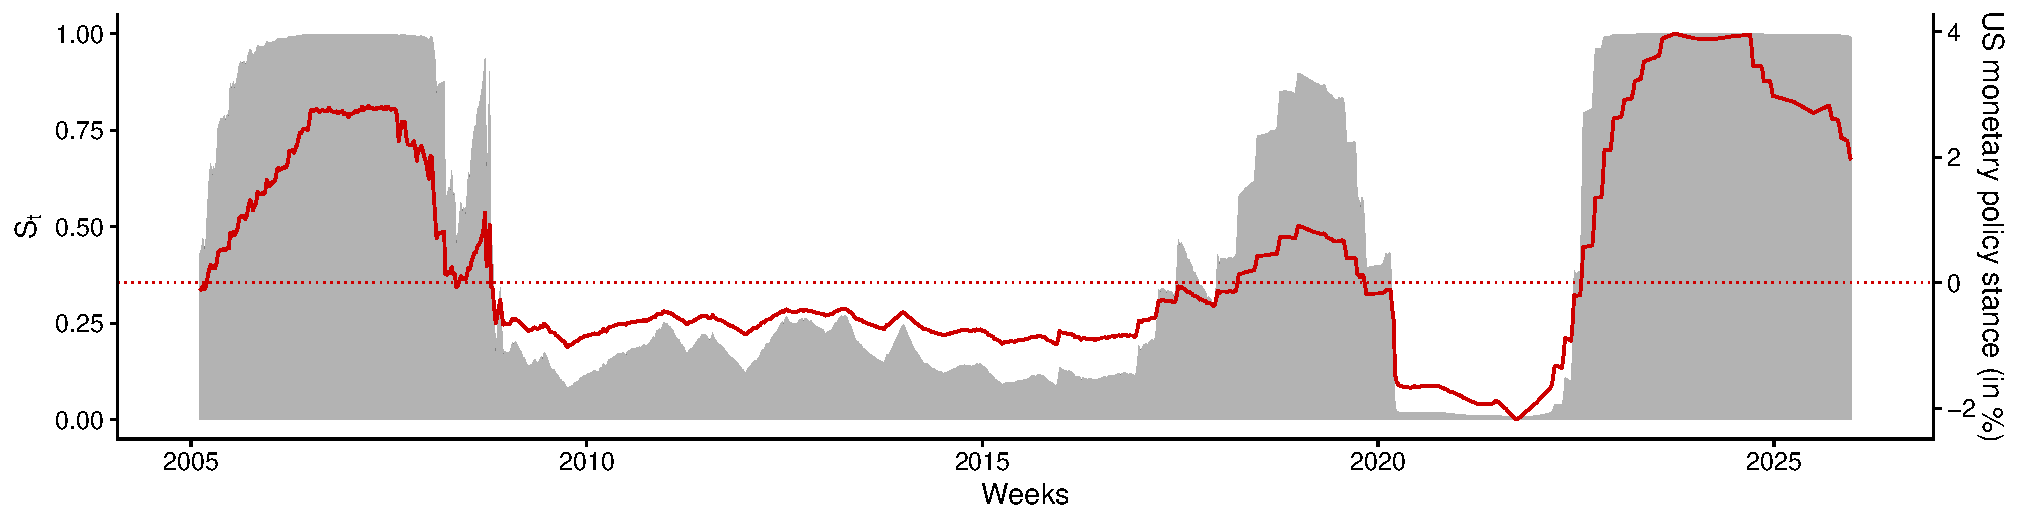
\includegraphics[width= 1\textwidth]{images_updated/DIFF_EA_Motto/St.pdf}
\caption*{\footnotesize \textit{Notes:} Gray areas denote the posterior mean of $S_t$, the transition function, where 0 (1) indicates an expansive (restrictive) regime\rev{; the darker shading marks the 68\% posterior credible band}. The red line depicts the constructed US monetary policy indicator in percent, as defined in \autoref{sec:measuring}\rev{, with the dotted line marking the neutral stance (zero), at which the calibrated transition function crosses $S_t = 0.5$. Estimated on the full 2005--2025 sample (specification \texttt{main} in the replication code \texttt{Codes/STVARestimation.R}); the swap-augmented system covers the entire sample thanks to the 2026 ILS data update. The state allocation is invariant to the outlier exclusion described in \autoref{sec:measuring}, since it depends only on the US stance and the calibrated transition parameters.}}\end{figure}
Given the gradual improvement in US economic conditions from 2013, the Fed began to scale back some of the expansionary measures, most notably through the tapering of the third large-scale asset purchase program, which began in January and ended in October 2014. The Fed's balance sheet remained at the same level until the fall of 2017, when the Fed began a slow unwinding. In addition, the December 2015 FOMC meeting marked a period where the Fed decided to gradually raise interest rates. This led to a gradual tightening with one hike in 2016, three hikes in 2017, and four hikes in 2018, each by 25 basis points. \rev{This hiking cycle lifts the policy rate above the natural rate in the spring of 2018, and $S_t$ accordingly moves into restrictive territory (annual averages of about $0.7$ in 2018--2019)---a mildly restrictive interlude that ends when the Fed's insurance cuts push the stance back below neutral in late 2019. The model then places the COVID-19 episode firmly in the expansionary regime, with $S_t$ falling essentially to zero in 2021. The most informative episode for our purposes, however, is the most recent one: in response to the post-pandemic inflation surge the Fed tightened sharply, the stance crosses neutral in mid-2022, and $S_t$ remains pinned at unity from 2023 through the end of 2025, mirroring---and in both magnitude and duration exceeding---the restrictive phase of 2006--2007. This is the first pronounced restrictive-Fed episode in our sample that occurs outside a recession and away from the effective lower bound, and it is precisely this variation that sharpens the identification of the state-dependent responses discussed below. Equipped with this information, we now proceed with the dynamic analysis.}

